\documentclass[tikz,border=12pt]{standalone}
\usepackage[T1]{fontenc}
\usepackage{mathpazo}
\usepackage{amsmath,amssymb}
\usetikzlibrary{arrows.meta, positioning, calc, decorations.pathreplacing}

\definecolor{stblue}{HTML}{7B97AD}
\definecolor{rwgold}{HTML}{B8995E}
\definecolor{sage}{HTML}{7A9A7E}
\definecolor{dkbrown}{HTML}{3D3530}
\definecolor{wmgray}{HTML}{7B7067}
\definecolor{cream}{HTML}{F9F6F0}
\definecolor{border}{HTML}{D4C9B8}
\definecolor{terracotta}{HTML}{C47A6A}

\begin{document}
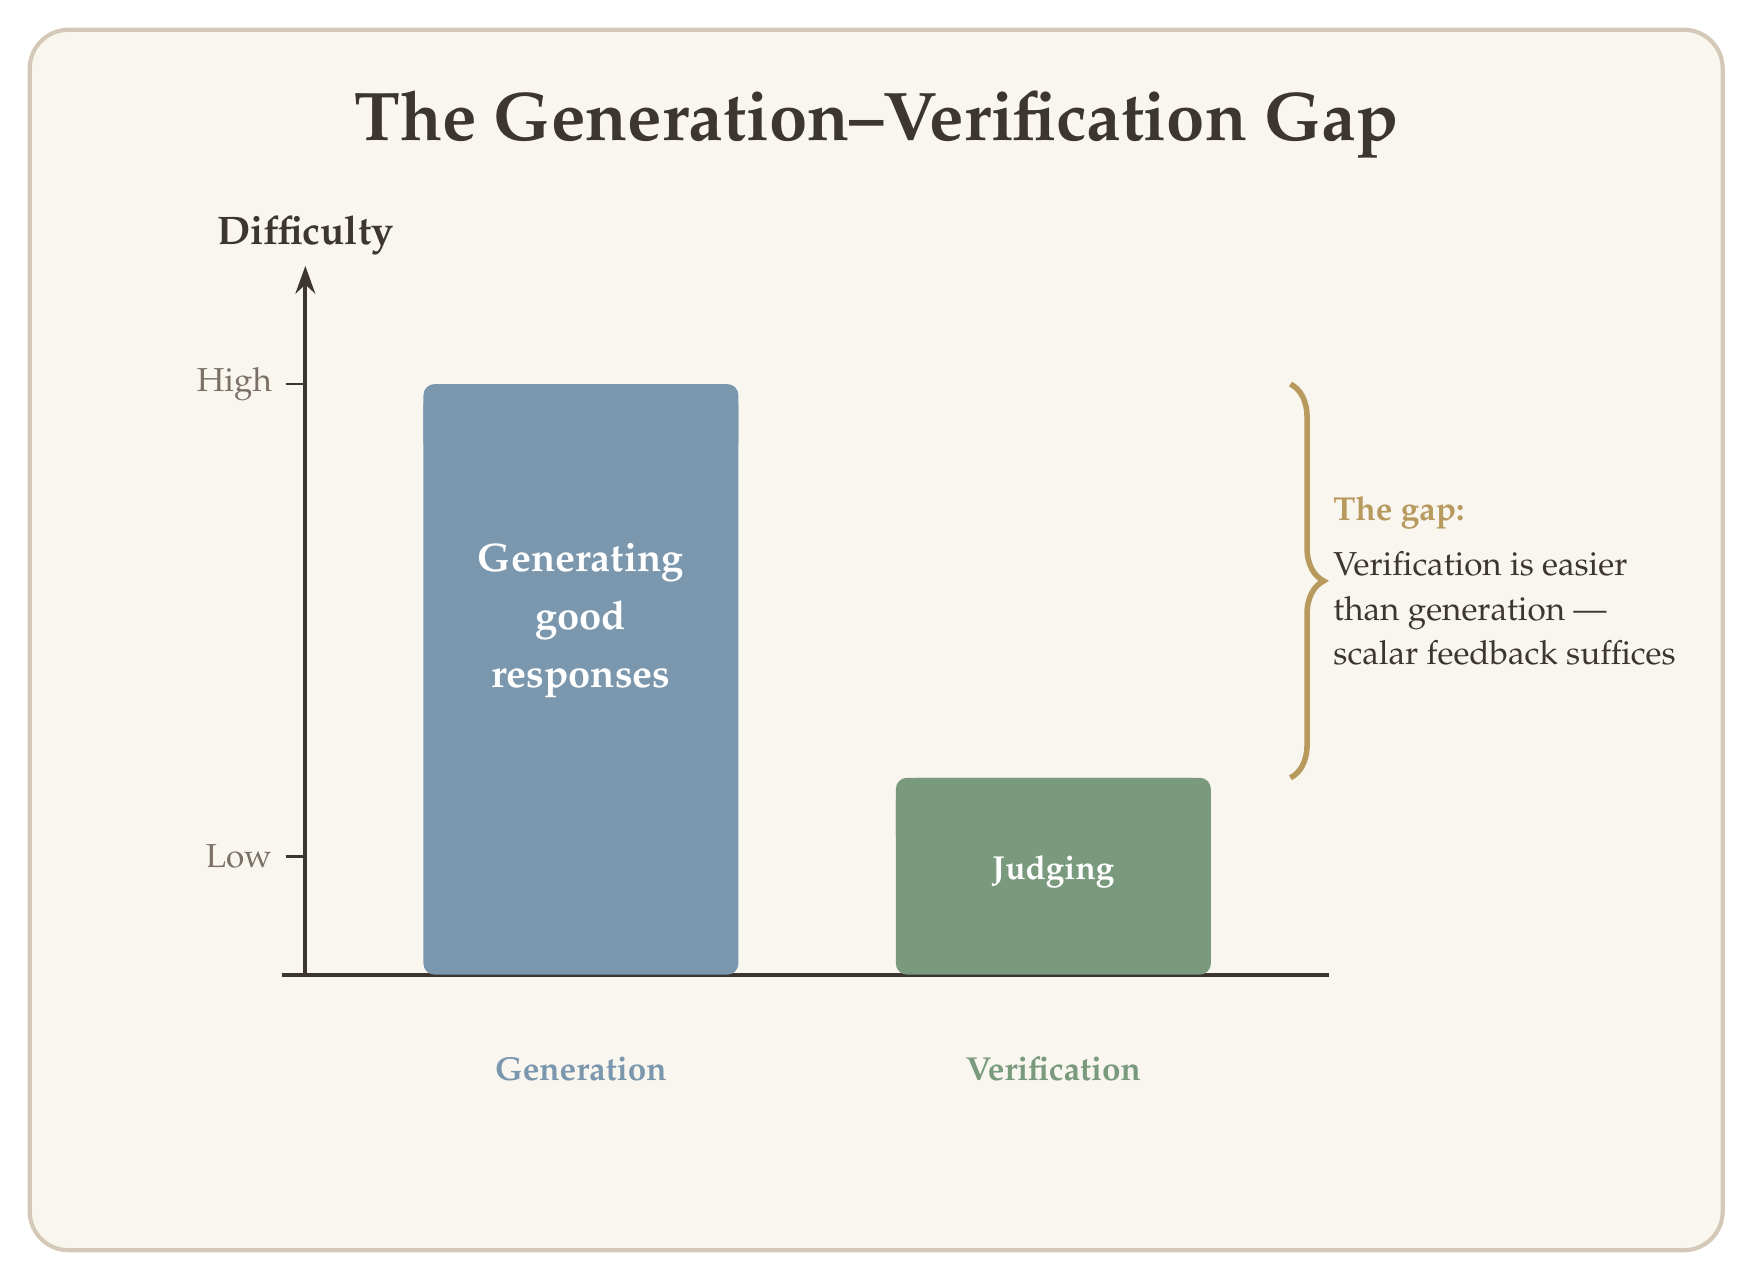
\begin{tikzpicture}[
  >={Stealth[length=3.5mm, width=2.5mm]},
  brace/.style={decorate, decoration={brace, amplitude=12pt, raise=6pt},
    line width=2pt, rwgold},
]

% Background
\fill[cream, rounded corners=14pt] (-3.5,-3.5) rectangle (18,12);
\draw[border, rounded corners=14pt, line width=1.5pt] (-3.5,-3.5) rectangle (18,12);

% Title
\node[font=\Huge\bfseries, text=dkbrown] at (7.25,10.8)
  {The Generation--Verification Gap};

% =============================================
% Axes
% =============================================

% Y-axis
\draw[dkbrown, line width=1.5pt, ->] (0,0) -- (0,9)
  node[above, font=\Large\bfseries, text=dkbrown] {Difficulty};

% X-axis
\draw[dkbrown, line width=1.5pt] (-0.3,0) -- (13,0);

% Y-axis ticks
\draw[dkbrown, line width=1pt] (-0.25,1.5) -- (0,1.5);
\node[left, font=\large, text=wmgray] at (-0.3,1.5) {Low};

\draw[dkbrown, line width=1pt] (-0.25,7.5) -- (0,7.5);
\node[left, font=\large, text=wmgray] at (-0.3,7.5) {High};

% =============================================
% Bars
% =============================================

% Bar 1: Generation (tall)
\fill[stblue, rounded corners=4pt]
  (1.5,0) rectangle (5.5,7.5);
% Rounded top overlay
\fill[stblue, rounded corners=8pt]
  (1.5,6.5) rectangle (5.5,7.5);

% Bar 2: Verification (short)
\fill[sage, rounded corners=4pt]
  (7.5,0) rectangle (11.5,2.5);
% Rounded top overlay
\fill[sage, rounded corners=8pt]
  (7.5,1.5) rectangle (11.5,2.5);

% =============================================
% Bar labels
% =============================================

% Inside tall bar
\node[font=\Large\bfseries, text=white, align=center] at (3.5,4.5)
  {Generating\\[3pt]good\\[3pt]responses};

% Inside short bar
\node[font=\large\bfseries, text=white, align=center] at (9.5,1.3)
  {Judging};

% Below bars: category labels
\node[font=\large\bfseries, text=stblue, align=center] at (3.5,-1.2)
  {Generation};

\node[font=\large\bfseries, text=sage, align=center] at (9.5,-1.2)
  {Verification};

% =============================================
% Bracket showing the gap
% =============================================

\draw[brace]
  (12.3,7.5) -- (12.3,2.5);
\node[right=18pt, font=\large, text=dkbrown, align=left] at (12.3,5.0)
  {{\bfseries\color{rwgold}The gap:}\\[6pt]
   Verification is easier\\[2pt]
   than generation ---\\[2pt]
   scalar feedback suffices};

\end{tikzpicture}
\end{document}
